\chapter{Rotation \& angular momentum}

%图1.1
\begin{comment}
\begin{figure}[ht]
    \centering
    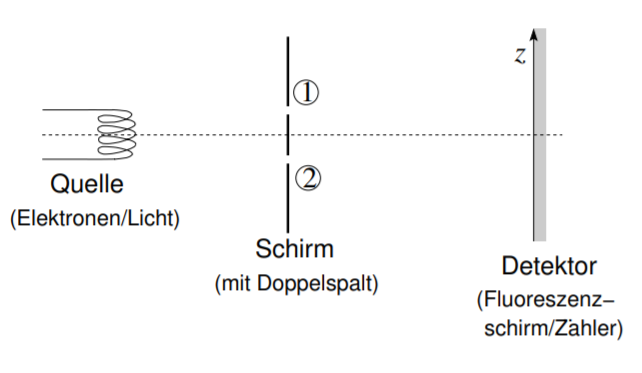
\includegraphics[scale=1]{1_1.PNG}
    \captionsetup{font={Large}}
    \caption{The double-slit experiment: those emitted by the source particles/waves hit a screen with two overlays columns and are analyzed in the detector.}
    \label{fig:1.1}
\end{figure}
\\
\end{comment}

Symmetries play an important role in physics, especially in quantum mechanics. They not only allow the classification of solutions but also simplify their calculation. To get started, let's start with the translations, a simple and important symmetry operation.

\section{Translation}
Let $\Psi(\vec{r})$ be a wave function in the place representation, eg, a wave packet at $\vec{ r} = 0$. An (active) shift of the packet by $\vec{a}$ is achieved by the operation $\Psi(\vec{r})\to\Psi(\vec{r}-\vec{a})$, see fig. 4.1. We denote the translation $\vec{r}\to\vec{r}+\vec{a}$ in real space with $T_{\vec{a}}\vec{r}=\vec{r}+\vec{a}$. The picture in the Hilbert space
%公式 4.1
\begin{equation}
\begin{aligned} U_{\vec{a}}: \mathcal{H} & \rightarrow \mathcal{H} \\\left(U_{\vec{a}} \Psi\right)(\vec{r}) &=\Psi\left(T_{\vec{a}}^{-1} \vec{r}\right) \\ &=\Psi(\vec{r}-\vec{a}) \end{aligned}
\end{equation}
generates a representation\footnote{$\left(U_{\vec{a}} \Psi\right)(\vec{r})=\Psi\left(T_{\vec{a}} \vec{r}\right)$ creates an anti representation. For an illustration applies
$\left[U_{a} \Psi\right](x)=\Psi\left(T_{a}^{-1} x\right):\left[U_{a} U_{b} \Psi\right](x)=\left[U_{a} \Phi\right](x)=\Phi\left(T_{a}^{-1} x\right)$ in which $\Phi(x)=\left[U_{b} \Psi\right](x)=$
$\Psi\left(T_{b}^{-1} x\right)$ and together $\left[U_{a} U_{b} \Psi\right](x)=\Psi\left(T_{b}^{-1} T_{a}^{-1} x\right)=\Psi\left(\left(T_{a} T_{b}\right)^{-1} x\right),$ or $\left\langle x\left|U_{a} U_{b}\right| \Psi\right\rangle=$
$\left\langle T_{a}^{-1} x\left|U_{b}\right| \Psi\right\rangle=\left\langle T_{b}^{-1} T_{a}^{-1} x | \Psi\right\rangle=\left\langle\left(T_{a} T_{b}\right)^{-1} x | \Psi\right\rangle$} of the (abelian) group $G_T = {T_{\vec{a}}| \vec{a} \in \mathbb{R}^3}$ of the translations in $\mathbb{R}^3$ in the Hilbert space $\mathcal{H}$ of the wave functions. We call this representation $\mathcal{G}_{T}=\left\{U_{\vec{a}} | T_{\vec{a}} \in G_{T}\right\}$. The location representation for the operators $U_{\vec{a}}$ can be easily found,
%公式 4.2
\begin{equation}
\begin{aligned}
    \left(U_{\vec{a}} \Psi\right)(\vec{r}) &=\Psi_{\vec{a}}(\vec{r})=\Psi(\vec{r}-\vec{a}) \\ 
    &\overset{\vec{a}\text{ small }}{\approx}  \Psi(\vec{r})-\vec{a} \cdot(\vec{\nabla} \Psi)(\vec{r}) \\ 
    &=(11-i \vec{a} \cdot \vec{p} / \hbar) \Psi(\vec{r}) \\ 
    & \approx e^{-i \vec{a} \cdot \vec{p} / \hbar} \Psi(\vec{r}) \end{aligned}
\end{equation}
The result $(4.2)$ is exactly: $(a)$ write $\Psi(\vec{r}-\vec{a})$ as a Taylor series and resummate, or $(b)$ integrate: first, choose an infinitesimal shift $\vec{a}\to\vec{a}+\delta\vec{a}, \Psi_{\vec{a}+\delta \vec{a}}=\Psi_{\vec{a}}-(i \delta \vec{a} \cdot \vec{p} / \hbar) \Psi_{\vec{a}}$ and we get the differential equation $\partial_{\vec{a}} \Psi_{\vec{a}}=-i(\vec{p} / \hbar) \Psi_{\vec{a}}$; with the initial condition $\Psi_{\vec{0}}=\Psi$ we obtain via integration the solution $\Psi_{\vec{a}}=exp(-i\vec{p}\cdot\vec{a}/\hbar)\Psi_{\vec{0}}$. Thus, the translation operator has the form
%公式 4.3
\begin{equation}
    U_{\vec{a}}=e^{-i\vec{a}\cdot \vec{p}/\hbar}
\end{equation}
It describes the active translation/shift of the wave function by $\vec{a}$, where the momentum operator $\vec{p}$ is the infinitesimal origin of the translation. With $\vec{p}$ hermitian, $U_{\vec{a}}$ unitary. $\mathcal{G}_T$ and $G_T$ are abelian, continuously contiguous, three-parameter non-compact groups.
%图 4.1
\begin{figure}[ht]
    \begin{minipage}{0.5\textwidth}
        \centering
        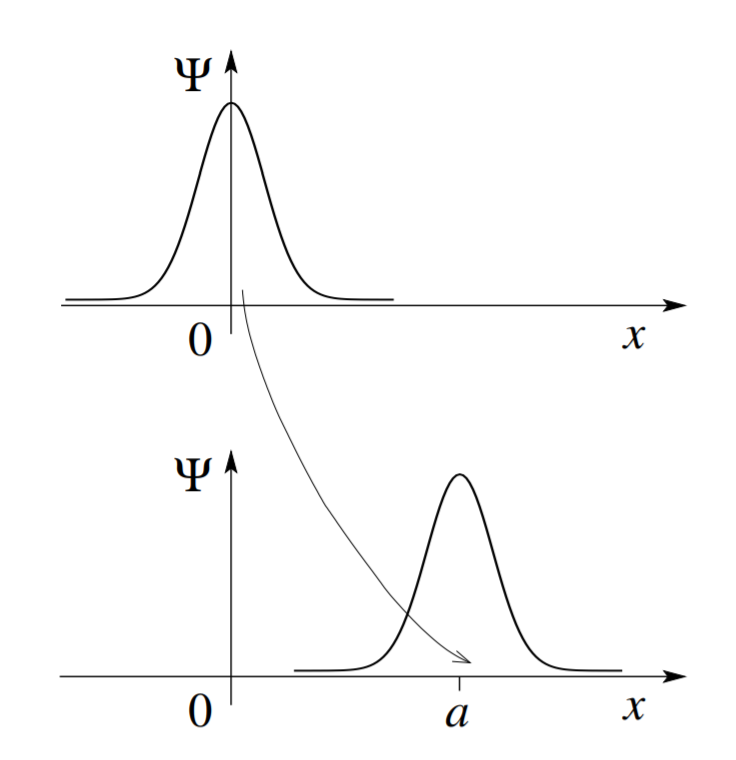
\includegraphics[scale=1]{4_1.PNG}
    \end{minipage}
    \begin{minipage}{0.5\textwidth}
        \captionsetup{font={Large}}
        \caption{Active translation of a (Gaussian) wave packet
        around $a, \Psi (x) \to \Psi (x - a) = (Ua\Psi) (x)$.}
    \end{minipage}
\end{figure}
The isomorphic groups $\mathcal{G}_T$ and $G_T$ are useful in describing a symmetry of the problem: If the Hamiltonian $H$ is translation invariant then $[H, U_{\vec{a}}] = 0$ for all $T_{\vec{a}}\in G_T$ and the operators $H$ and $U_{\vec{a}}\in\mathcal{G}_T$ have common eigenvectors. The use of such symmetries facilitates the solution of many problems, in particular the solution of eigenvalue problems like that of the periodic potential, cf. Chapter 3, where we used the symmetry of the discrete translation group. GT is an example of geometric symmetry.

\section{Rotation}
Another example of geometrical symmetry is the rotations $R_{\vec{w}} \in SO (3)$ with the rotation axis $\vec{w}$ and the rotation angle $0 \leq w \leq 2\pi$. The group $SO (3)$ is called a special orthogonal group (det = 1) in $\mathbb{R}^3$; it is not abelian, continuous (but not simple) coherent, tri-parametric, and compact, cf. see also fig. 4.2. The group operation $\circ$ is the matrix multiplication.
%图 4.2
\begin{figure}[ht]
    \centering
    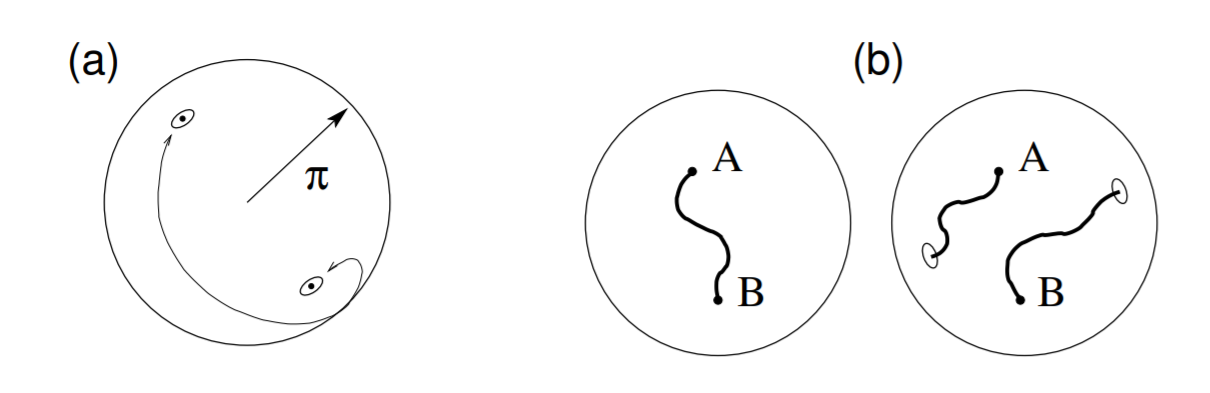
\includegraphics[scale=1]{4_2.PNG}
    \captionsetup{font={Large}}
    \caption{$(a)$ The special orthogonal group $SO (3)$ can be parameterized by vectors in the sphere with radius $\pi$, whereby opposite points on the surface can be identified. $(b)$ The group is not simply connected: the two paths from A to B combine to form a loop that can not be contracted.}
\end{figure}
We denote the unitary representation of the rotation $R_{\vec{w}} \in SO (3)$ by $\vec{w}$ in the Hilbert space of the one-particle wave functions $\Psi (\vec{r})$ with $U_{\vec{w}}$,
%公式 4.4
\begin{equation}
    \left(U_{\vec{\omega}} \Psi\right)(\vec{r})=\Psi_{\vec{\omega}}(\vec{r})=\Psi\left(R_{\vec{\omega}}^{-1} \vec{r}\right)
    \end{equation}
the rotation operator $U _{\vec{w}}$ turns the wave function by $\vec{w}$. Again, if the Hamiltonian is invariant under rotations (e.g., $V (\vec{r}) = V (r)$, a central potential) then $[H, U_{\vec{w}}] = 0$ for all $R_{\vec{w}}\in SO (3)$. Note, however, that the rotations $R_{\vec{w}}$ do not commute among themselves (i.a.). Nevertheless, the $SO (3)$ symmetry is again extremely helpful (though not entirely trivial) in solving many problems, such as finding the eigenbase as a three-invariant operator. Note that the Coulomb potential $-\kappa / r$ has not only the geometric symmetry $SO (3)$ but an additional dynamic symmetry. This symmetry is associated with the Lenz vector $\vec{M} = \vec{p} \wedge \vec{L} / \mu - \kappa \vec{r} / r$ and is responsible for the formation of the closed elliptical orbits in the Kepler problem (for any central potential, the orbits would not be closed $\Rightarrow \vec{M} = \text{ constant}$.). The symmetry of the Kepler problem is given by the group $SO (4)$, more later. For small rotations $R_{\vec{w}}^{-1}\vec{r}\approx\vec{r}-\vec{w}\wedge\vec{r}$ and in analogy to (4.2) we find
%公式 4.5
\begin{equation}
\begin{aligned} \Psi_{\vec{\omega}}(\vec{r}) & \approx \Psi(\vec{r}-\underbrace{\vec{\omega} \wedge \vec{r}})=\Psi(\vec{r})-\varepsilon_{i j k} \omega_{i} r_{j} \partial_{k} \Psi(\vec{r})+\cdots \\ &=[1]-i \vec{\omega} \cdot \vec{L} / \hbar+\cdots] \Psi(\vec{r})=e^{-i \vec{\omega} \cdot \vec{L} / \hbar} \Psi(\vec{r}) \\ \vec{L} &=\vec{r} \wedge \vec{p} \quad \Leftrightarrow \quad L_{i}=\varepsilon_{i j k} r_{j}\left(-i \hbar \partial_{k}\right) \end{aligned}
\end{equation}
The representation $U_{\vec{w}}=exp(-i\vec{w}\cdot\vec{L}/\hbar)$ holds for large $\vec{w}$: be $\vec{r}_{\vec{w}}=R^{-1}_{\vec{w}}\vec{r}$, then $\vec{r}_{\vec{w}+\delta\vec{w}}=\vec{r}_{\vec{w}}-\hat{w}\wedge\vec{r}_{\vec{w}}\delta\vec{w}$ with $\delta\vec{w}$ parallel to $\vec{w}$ and $ \hat{w} \equiv \vec{w} / w$. We get the differential equation
%公式 4.6
\begin{equation}
    \frac{\partial \Psi_{\vec{\omega}}}{\partial \omega}=-\frac{i}{\hbar} \hat{\omega} \cdot \vec{L} \Psi_{\vec{\omega}}
    \end{equation}
with $\Psi_0=\Psi$, and the integration yields
%公式 4.7
\begin{equation}
    \Psi_{\vec{\omega}}(\vec{r})=U_{\vec{\omega}} \Psi(\vec{r})=e^{-i \vec{\omega} \cdot \vec{L} / \hbar} \Psi(\vec{r})
    \end{equation}
The operator $\vec{L}=\vec{r}\wedge\vec{p}$ is the angular momentum operator (compare correspondence principle) and is the infinitesimal generatrix of the rotation
%公式 4.8
\begin{equation}
    U_{\vec{\omega}}=e^{-i \vec{\omega} \cdot \vec{L} / \hbar} \in \mathcal{S O}(3)
    \end{equation}
The groups $SO (3)$ and their representation $SO (3)$ in Hilbert space $\mathcal{H}$ are isomorphic.
Instead of the states $\Psi$ we can also shift or rotate the operators $A$: With $\langle\Psi, A \Psi\rangle=\left\langle\Psi_{\vec{a}}, A_{\vec{a}} \Psi_{\vec{a}}\right\rangle=\left\langle\Psi, U_{\vec{a}}^{\dagger} A_{\vec{a}} U_{\vec{a}} \Psi\right\rangle$ (simultaneous shifts / rotations of $A$ and $\Psi$ pick up) can be found immediately

%公式 4.9
\begin{equation}
\begin{aligned} A_{\vec{a}} &=e^{-i \vec{a} \cdot \vec{p} / \hbar} A e^{i \vec{a} \cdot \vec{p} / \hbar} \quad \text { and as well } \\ A_{\vec{\omega}} &=e^{-i \vec{\omega} \cdot \vec{L} / \hbar} A e^{i \vec{\omega} \cdot \vec{L} / \hbar} \end{aligned}
\end{equation}
In diracnotation we write for the formula (4.5)
%公式 4.10
\begin{equation}
\begin{aligned}\left\langle T_{\vec{a}}^{-1} \vec{r}\right| &=\left\langle\vec{r}-\vec{a}\left|=\langle\vec{r}| e^{-i \vec{a} \cdot \vec{p} / \hbar}\right.\right.\\\left\langle R_{\vec{\omega}}^{-1} \vec{r}\right| &=\left\langle\vec{r}_{\vec{\omega}}\left|=\langle\vec{r}| e^{-i \vec{\omega} \cdot \vec{L} / \hbar}\right.\right.\end{aligned}
\end{equation}

\section{Angular momentum}
We can use the expression for the angular momentum
%公式 4.11
\begin{equation}
    \vec{L}=\vec{r} \wedge \vec{p}
    \end{equation}
derive either from the principle of correspondence or as infinitesimal generators of rotation. With $L_{i}=\varepsilon_{i j k} x_{j}(-i \hbar) \partial_{k}$ we find $(1 = x, 2 = y, 3 = z)$

%公式 4.12
\begin{equation}
\begin{aligned} 
    L_{x}=y p_{z}-z p_{y}, \quad L_{x}^{\dagger}&=L_{x} \\ 
    L_{y}=z p_{x}-x p_{z}, \quad L_{y}^{\dagger}&=L_{y} \\ 
    L_{z}=x p_{y}-y p_{x}, \quad L_{z}^{\dagger}&=\left(x p_{y}\right)^{\dagger}-\left(y p_{x}\right)^{\dagger} \\ 
    &=p_{y}^{\dagger} x^{\dagger}-p_{x}^{\dagger} y^{\dagger}=p_{y} x-p_{x} y \\ &=x p_{y}-y p_{x}=L_{z} \end{aligned}
\end{equation}
The angular momentum operator $\vec{L} = \vec{L}^{\dagger}$ is Hermitian and hence the rotation operators $U_{\vec{w}}=exp[-i\vec{w}\cdot\vec{L}/\hbar]$ are unitary. It becomes interesting when we consider different commutation relations ($\hat{n}$ ​​the unit vector in the direction $\vec{n}$),
%公式 4.13
%公式 4.14
%公式 4.15
%公式 4.16
\begin{eqnarray}
    \text { with the place: }  \quad \left\{\begin{array}{lcl}
            {\left[L_{i}, x_{j}\right]} & {=} & {i \hbar \varepsilon_{i j k} x_{k}} \\ 
            {\left[\hat{n} \cdot \hat{L}, \vec{r}\right]} & {=} & {i \hbar \hat{r} \wedge \hat{n}}
        \end{array}\right.\\
    \text { with the impulse: } \quad \left\{\begin{array}{lcl}
            {\left[L_{i}, p_{j}\right]} & {=} & {i \hbar \varepsilon_{i j k} p_{k}} \\ {[\hat{n} \cdot \vec{L}, \vec{p}]} & {=} & {i \hbar \vec{p} \wedge \hat{n}_{k}}
        \end{array}\right.\\
    \text { with yourself: } \quad \left\{\begin{array}{lcl}
            {\left[L_{i}, L_{j}\right]} & {=} & {i \hbar \varepsilon_{i j k} L_{k}} \\ 
            {\left[\hat{n} \cdot \vec{L}, \vec{L}\right]} & {=} & {i \hbar \vec{L} \wedge \hat{n}} \\ {\vec{L} \wedge \vec{L}} & {=} & {i \hbar \vec{L}}
        \end{array}\right.
\end{eqnarray}

\begin{equation}
        \text{ with a scalar: } \qquad \left[\vec{L}, A \right] = \quad 0
\end{equation}
Proof by calculating: $\left[L_{x}, x\right]=\left[y p_{z}-z p_{y}, x\right],$ everything involves different directions $\rightarrow=0 ;\left[L_{x}, y\right]=\left[y p_{z}-z p_{y}, y\right]=-z\left[p_{y}, y\right]=i \hbar z ;\left[L_{x}, z\right]=\left[y p_{z}-z p_{y}, z\right]\\=y\left[p_{z}, z\right]=-i \hbar y,$ thus is $\left[L_{x}, x_{j}\right]=i \hbar \varepsilon_{1 j k} x_{k},$ cyclic exchange leads to $\left[L_{i}, x_{j}\right]=i \hbar \varepsilon_{i j k} x_{k} .$ The multiplication by $\hat{n}_{i}$ gives $[\hat{n} \cdot \vec{L}, \vec{r}]=i \hbar \vec{r} \wedge \hat{n} .$ All other printouts are also calculated.
An alternative and elegant proof can be found by considering the effect of small rotations on vector operators. Let $\vec{A}$ be a vector operator (i.e., the components of $\vec{A}$ behave like a vector under rotation), then
%公式 4.17
\begin{equation}
    \vec{A}_{\vec{w}} \quad \approx \quad \vec{A} - \vec{w}\wedge \vec{A}
\end{equation}
for small turns around $\vec{w}$. On the other hand, from (4.9)
%公式 4.18
\begin{equation}
\begin{aligned} \vec{A}_{\vec{\omega}} &=e^{-i \vec{\omega} \cdot \vec{L} / \hbar} \vec{A} e^{i \vec{\omega} \cdot \vec{L} / \hbar} \approx(11-i \vec{\omega} \cdot \vec{L} / \hbar) \vec{A}(11+i \vec{\omega} \cdot \vec{L} / \hbar) \\ & \approx \vec{A}-(i / \hbar) \omega_{i}\left[L_{i}, \vec{A}\right] \end{aligned}
\end{equation}
The comparison with the above expression (4.17) yields $(i/\hbar)w_l[L_l,A_j]=\varepsilon_{jkl}w_lA_k; [\vec{w}\cdot\vec{L},\vec{A}]=i\hbar\vec{A}\wedge\vec{w}$. The operators $\vec{x},\vec{p},\vec{L}$ are vector operators, which immediately follows the formulas (4.13) - (4.15).

\section{Eigenvalues ​​and eigenvectors}
We work out a formal solution of the eigenvalue problem for a vector operator with the properties

%公式 4.19
\begin{equation}
    \vec{L} \text{ hermitean, } \quad \vec{L}\wedge\vec{L}=i\hbar\vec{L}
\end{equation}
The relations (4.19) fully characterize the angular momentum. The three components Li do not commute in pairs, so there is no common eigenbasis. But $L^2=\vec{L}\cdot\vec{L}$ is a rotation scale, so $[L^2, \vec{L}] = 0$. Hence, we can diagonalize $L^2$ and a component of $\vec{L}$ simultaneously. We choose $L_z$. Note: With $L_z$ sharp surely $L_x, L_y$ is out of focus, since $[L_x, L_z] = -i\hbar\vec{L_y}, [L_y, L_z] = i\hbar \vec{L_x}$. The operator $L^2$ is positive, $\left\langle\Psi, L^{2} \Psi\right\rangle=\left\langle\Psi, L_{i} L_{i} \Psi\right\rangle \geq 0$, so the eigenvalues ​​of $L^2$ are positive and we make the approach $\hbar^2l (l + 1), l ≥ 0$ (note $[L] = [xp]$ is an effect). The eigenvalues ​​of $L_z$ have the form $\hbar m$, where $m$ denotes the azimuthal quantum number. The formal eigenbasis to $L^2$ and $L_z$ is thus the set {$| l, m\rangle$}

%公式 4.20
\begin{equation}
\begin{aligned} L^{2}|l, m\rangle &=\hbar^{2} l(l+1)|l, m\rangle \\ L_{z}|l, m\rangle &=\hbar m|l, m\rangle \end{aligned}
\end{equation}
we have to find the allowed values ​​for $l$ and $m$. Our approach follows the strategy used in the harmonic oscillator. We drove up and down operators $L_{\pm}$
%公式 4.21
\begin{equation}
    L_{+}\equiv L_x+iL_y,\quad L_{-}\equiv L_x-iL_y
\end{equation}
and consider their rules of confusion,
%公式 4.22
\begin{equation}
\begin{aligned}\left[L_{z}, L_{\pm}\right] &=\left[L_{z}, L_{x} \pm i L_{y}\right]=i \hbar\left(L_{y} \mp i L_{x}\right) \\ &=\hbar\left(\pm L_{x}+i L_{y}\right)=\pm \hbar L_{\pm} \end{aligned}
\end{equation}
The commutator $[L_+, L^{\dagger}_+] = [L_+, L_-] = 2 \hbar L_z$ follows
%公式 4.23
\begin{equation}
    L_{\pm} L_{\mp}=L_{x}^{2}+L_{y}^{2} \mp i\left(L_{x} L_{y}-L_{y} L_{x}\right)=L^{2}-L_{z}^{2} \pm \hbar L_{z}
    \end{equation}
Thus, the pairs $L_z, L_{\pm}$ play the same role as $N, a^{\dagger}$ and $N, a: L_+$ is an ascending operator for $L_z$, while $L_-$ plays the role of the descending operator; this is also consistent with the relationship $L^{\dagger}_+ = L_-$. Compared to the operators $a, a^{\dagger}$, and $N = a^{\dagger} a$ in the harmonic oscillator problem (see (3.118))
%公式
$$[a,a^{\dagger}]=1, \quad [N,a^{\dagger}]=a^{\dagger}, \quad [N,a]=-a$$
satisfy the operators $L_{\pm}$, and $L_z$ following relationships
%公式 4.24
\begin{equation}
    \left[L_{-}, L_{+}\right]=-2 \hbar L_{z}, \quad\left[L_{z}, L_{+}\right]=\hbar L_{+}, \quad\left[L_{z}, L_{-}\right]=-\hbar L_{-}
    \end{equation}
Note that the commutator $[L_-, L^{\dagger}_+] = -2\hbar L_z$ is manifestly different from its analog $[a, a^{\dagger}] = 1$ in the harmonic oscillator problem; also, $N = a^{\dagger} a$ but $\hbar L_z  \neq L_+ L_-$; the important properties for the application of ascending and descending operators are given by (4.24).
%图 4.3
\begin{figure}[ht]
    \begin{minipage}{0.5\textwidth}
        \centering
        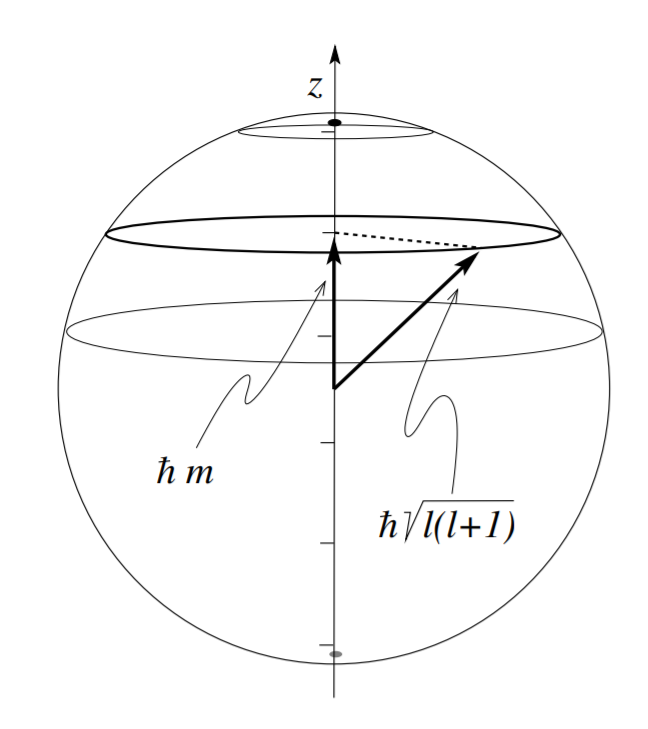
\includegraphics[scale=1]{4_3.PNG}
    \end{minipage}
    \begin{minipage}{0.5\textwidth}
        \captionsetup{font={Large}}
        \caption{The system with angular momentum $L = \hbar\sqrt{l (l + 1)}$ has a sharp component along the $z-$axis with allowed values $L_z = m\hbar, -l\leq m\leq l$, and undeterminated components $L_x$ and $L_y$ in the $xy$ plane.}
    \end{minipage}
\end{figure}
We verify that $L_{\pm}$ are really up and down operators for eigenstates of $L_z$,
%公式 4.25
\begin{equation}
\begin{aligned} L_{z} L_{\pm}|l, m\rangle &=\left(L_{\pm} L_{z}+\left[L_{z}, L_{\pm}\right]\right)|l, m\rangle= L_{\pm}\left(L_{z} \pm \hbar\right)|l, m\rangle \\ &=\hbar(m \pm 1) L_{\pm}|l, m\rangle \end{aligned}
\end{equation}
The states $L_{\pm} | l,m\rangle$ thus agree with the states $| l, m \pm 1\rangle$, except for normalization. With the help of normalization conditions (we use (4.23))
%公式
$$\left\langle l, m\left|L_{\pm} L_{\mp}\right| l, m\right\rangle=\hbar^{2}[l(l+1)-m(m \mp 1)]=\left|c_{l, m}^{\mp}\right|^{2}\langle l, m \mp 1 | l, m \mp 1\rangle$$
we find the new eigenvectors $| l, m \pm 1\rangle$ to $L_z$,
%公式 4.26
\begin{equation}
    |l, m \pm 1\rangle= L_{\pm}|l, m\rangle / \hbar \sqrt{l(l+1)-m(m \pm 1)}
    \end{equation}
To find the spectrum, let's look again through the $L_+$ and $L_-$ produced conditions, in particular their norm. It is
%公式 4.27
\begin{equation}
    \left\langle l, m\left|L_{\pm} L_{\mp}\right| l, m\right\rangle=\hbar^{2}[l(l+1)-m(m \mp 1)] \geq 0
    \end{equation}
Thus, $(l + 1/2)^2 \geq (m \pm 1/2)^2$ and we get the restriction
%公式 4.28
\begin{equation}
    -l\leq m \leq l.
\end{equation}
Suppose that $m> 1$, then $(m + 1/2)^2> (l + 1/2)^2$ and we find a contradiction. Let $m <-l$ then $(m - 1/2)^2> (-l - 1/2)^2 = (l + 1/2)^2$ and again we find a contradiction. The iterative application of $L_+$ and $L_-$ must be constrained by the condition (4.28), so that both $l (l + 1) - m (m + 1)$ for the largest $m$ and $l (l + 1 ) - m (m - 1)$ for the smallest $m$ disappear. Obviously, $m_{max} = 1$ and $m_min = -l$. But since mmax follows from mmin by addition of ones, $l$ must be either half or integer. Thus, $m$ can take the following values:
%公式 4.29
\begin{equation}
\begin{array}{l}{m=-l,-l+1,-l+2, \cdots, 0, \cdots, l-2, l-1, l ; \quad l \text { integer }} \\ {m=-l,-l+1, \cdots,-\frac{1}{2}, \frac{1}{2}, \cdots, l-2, l-1, l ; \quad l \text { half-integer. }}\end{array}
\end{equation}
These formal considerations provide us with the solution of the eigenvalue problem to the operators $L^2, L_z$ in the form:
%公式 4.30
\begin{equation}
\begin{array}{l}{L^{2}|l, m\rangle=\hbar^{2} l(l+1)|l, m\rangle \quad \text { mit } \quad l=n \text { oder } n+1 / 2, n \geq 0} \\ {L_{z}|l, m\rangle=\hbar m|l, m\rangle \quad \text { mit } \quad m=-l,-l+1, \ldots, l-1, l}\end{array}
\end{equation}
The eigenspace to $l$ is $2l + 1$-fold degenerate. We give this result the following physical interpretation: Let a system with angular momentum $L = \hbar\sqrt{l (l + 1)}$ be given. We can measure the angular momentum component $L_z$ along an axis (without limiting the generality, we choose the $z$-axis) without disturbing the value of $L^2$. The values ​​for $L_z$ lie between $-l \hbar$ and $l \hbar$ and can be changed into quanta of $\hbar$. The values ​​for the transverse components $L_x$ and $L_y$ are indeterminate, see Figure 4.3, a consequence of the non-interchangeability of $L_z$ with $L_x$ and $L_y$.\\\\
The $| l, m\rangle$ form an orthonormalized system: $\langle l, m | l_0, m_0 \rangle = \delta_{ll^{\prime}}\delta_{mm^{\prime}}$. With this we have found all the irreducible representations\footnote{The representations of $SO (3) / SU (2)$ belong to the all/half-number $l$} of the angular momentum Lie algebra. The $2l + 1$-dimensional representations are spanned by the states ${| l, m\rangle}$ with $L^2$ and $L_z$ diagonally. Some examples are shown in Table 4.1.

\section{Location}
The natural location representation for the angular momentum problem (or rotation) in $\mathbb{R}^3$ is the unitary sphere $S^2$. A location base is given by the angles $\theta, \varphi$ satisfy $|\theta, \varphi\rangle$ = state (of a particle) with sharp direction coordinates $\theta$ and $\phi$, cf. fig. 4.4. The space of the square integrable functions over the $\mathbb{R}^3$ can be decomposed according to $L^2 (\mathbb{R}^3) = L^2 (S^2) \otimes L^2 (R_+)$. The corresponding states to the position operator are written as $| \vec{r}\rangle$ and $| \theta, \phi, r\rangle$ in Cartesian and spherical coordinates.
%图 4.4
\begin{figure}[ht]
    \begin{minipage}{0.5\textwidth}
        \centering
        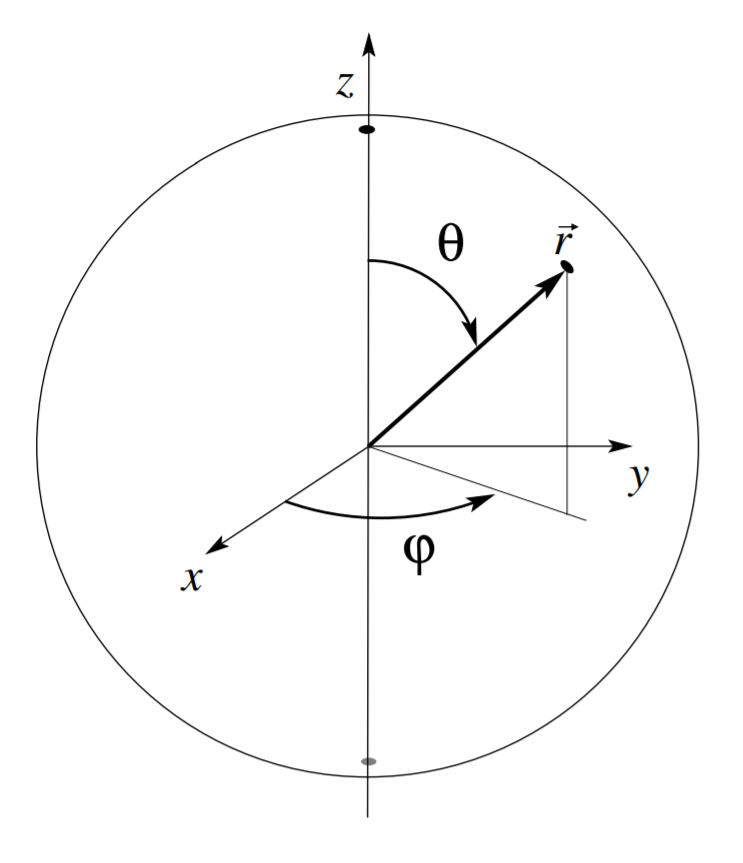
\includegraphics[scale=1]{4_4.PNG}
    \end{minipage}
    \begin{minipage}{0.5\textwidth}
        \captionsetup{font={Large}}
        \caption{Angular coordinates $\theta \in[0, \pi] \text{ and } \varphi \in [0, 2\pi)$.}
    \end{minipage}
\end{figure}
We want to represent the abstract vectors $|l,m\rangle$ in the $|\theta, \varphi\rangle$ basis. For this, we have to calculate the transformation matrices $\langle \theta, \varphi|l, m\rangle$. We need a location representation of the operators $L_z$ and $L^2$ and start with formula (4.10)
%公式 4.31
\begin{equation}
\begin{aligned}\left\langle R_{\vec{\omega}} \vec{r}\right| &=\langle\vec{r}| \exp (i \vec{\omega} \cdot \vec{L} / \hbar) \\ & \approx\langle\vec{r}| 1+i \vec{\omega} \cdot \vec{L} / \hbar \quad \text { for little ones } \vec{\omega} \\ & \approx\langle\vec{r}+\vec{\omega} \wedge \vec{r}| \end{aligned}
\end{equation}
We choose $r = 1, \vec{r}\in S^2$, and go to sphere coordinates
%公式 4:32
\begin{equation}
\left.\begin{array}{rl}{x} & {=\sin \theta \cos \varphi} \\ {y} & {=\sin \theta \sin \varphi} \\ {z} & {=\cos \theta}\end{array}\right\} \Leftrightarrow\langle\vec{r}|\rightarrow\langle\theta, \varphi|
\end{equation}
We are looking for a representation of the operators $L_z$ and $L_x$, $L_y$. First we write the differentials of Cartesian coordinates in spherical coordinates,
%公式 4:33
\begin{equation}
\left(\begin{array}{c}{d x} \\ {d y} \\ {d z}\end{array}\right)=\left(\begin{array}{c}{\cos \theta \cos \varphi d \theta-\sin \theta \sin \varphi d \varphi} \\ {\cos \theta \sin \varphi d \theta+\sin \theta \cos \varphi d \varphi} \\ {-\sin \theta d \theta}\end{array}\right)
\end{equation}
To find $L_z$ we choose $\vec{w} = (0, 0, w), w$ small; the associated rotation $R_{\vec{w}} \approx \vec{r} + \vec{w} \wedge \vec{r}$ produces a shift
%公式 4:34
\begin{equation}
\left(\begin{array}{l}{d x} \\ {d y} \\ {d z}\end{array}\right) \approx\left(\begin{array}{c}{-\omega y} \\ {\omega x} \\ {0}\end{array}\right)
\end{equation}
and by comparing (4.33) with (4.34) we find the differentials $d\theta = 0$ and $d\varphi = w$. Relation (4.31) then gives the representation of $L_z$ as a differential operator in spherical coordinates,
%公式 4:35
\begin{equation}
\begin{aligned}\langle\theta+ d \theta, \varphi+d \varphi| &=\left\langle\theta, \varphi+\omega\left|\approx\left\langle\theta, \varphi\left|+\omega \partial_{\varphi}\left\langle\theta, \varphi\left|=\langle\theta, \varphi|\left(11+i \omega L_{z} / \hbar\right)\right.\right.\right.\right.\right.\right.\\ & \Rightarrow L_{z}=-i \hbar \partial_{\varphi} \end{aligned}
\end{equation}
To find $L_x$ we choose $\vec{w} = (w, 0, 0), w$ small. The associated rotation in Cartesian coordinates yields

%公式 4:36
\begin{equation}
\left(\begin{array}{l}{d x} \\ {d y} \\ {d z}\end{array}\right) \approx\left(\begin{array}{c}{0} \\ {-\omega z} \\ {\omega y}\end{array}\right)
\end{equation}
and the comparison with (4.33) gives the differentials
%公式 4:37
\begin{equation}
\begin{aligned} d \theta &=-\omega \sin \varphi \\ d \varphi &=-\omega \cot \theta \cos \varphi \end{aligned}
\end{equation}
The evaluation of (4.31) for the rotation around $(w, 0, 0)$ gives us the operator $L_x$ in the form
%公式 4:38
\begin{equation}
\begin{aligned}
    &\langle\theta+ d \theta, \varphi+d \varphi|  \approx\langle\theta-\omega \sin \varphi, \varphi-\omega \cot \theta \cos \varphi| \\
    &=\left\langle\theta, \varphi\left|-\omega \sin \varphi \partial_{\theta}\left\langle\theta, \varphi\left|-\omega \cot \theta \cos \varphi \partial_{\varphi}\langle\theta, \varphi|\right.\right.\right.\right.\\
    &=\langle\theta, \varphi|] 1+i \omega L_{x} / \hbar \\ 
    &\Rightarrow L_{x}=-i \hbar\left(-\sin \varphi \partial_{\theta}-\cot \theta \cos \varphi \partial_{\varphi}\right) 
\end{aligned}
\end{equation}
Likewise we find $L_y$ and with $L^2 = L^2_x + L^2_y + L^2_z$ also $L^2$
%公式 4:39
\begin{equation}
    L_{y} =-i \hbar(\cos \varphi \partial_{\theta}-\cot \theta \sin \varphi \partial_{\varphi}) 
\end{equation}

%公式 4:40
\begin{equation}
    L^{2} =-\hbar^{2}\left[\frac{1}{\sin ^{2} \theta} \partial_{\varphi}^{2}+\frac{1}{\sin \theta} \partial_{\theta}\left(\sin \theta \partial_{\theta}\right)\right] 
\end{equation}
The up and down operators $L_{\pm}$ have the form
%公式 4:41
\begin{equation}
    L_{\pm}=-i \hbar e^{\pm i \varphi}\left(\pm i \partial_{\theta}-\cot \theta \partial_{\varphi}\right)
    \end{equation}
The Laplace operator in spherical coordinates can be written in the following form,
%公式 4:42
\begin{equation}
    \nabla^{2}=\frac{1}{r} \partial_{r}^{2} r-\frac{1}{r^{2}} \frac{L^{2}}{\hbar^{2}} \quad \text { with } L^{2} \operatorname{out}(4.40)
    \end{equation}
We can now calculate the eigenvectors $|l, m\rangle$ in the $|\theta,\varphi\rangle$ representation. First we determine the $\varphi$-dependence: It is $L_z | l, m\rangle = \hbar m | l, m\rangle$ and the projection on $|\theta,\varphi\rangle$ has the form
%公式 4:43
\begin{equation}
\begin{aligned}\left\langle\theta, \varphi\left|L_{z}\right| l, m\right\rangle &=\hbar m\langle\theta, \varphi | l, m\rangle \\ & \stackrel{(4,35)}{=}-i \hbar \partial_{\varphi}\langle\theta, \varphi | l, m\rangle \end{aligned}
\end{equation}
the integration over $\varphi$ yields
%公式 4:44
\begin{equation}
    \langle\theta, \varphi | l, m\rangle= e^{i m \varphi}\langle\theta, 0 | l, m\rangle
    \end{equation}
The result (4.44) is unique in $\mathbb{R}^3$ under the rotation $\varphi = 2\pi$ if $m$ is an integer; Accordingly, we consider here the basis functions for the irreducible representations of $SO (3)$ with $l$ integer (representations with integer $l$ have no unique basis functions). For the determination of the $\theta$-dependence we consider the relation $L_+ | l, l\rangle = 0$ and write these again on $|\theta,\varphi\rangle$,
%公式 4:45
\begin{equation}
\begin{aligned} 0=\left\langle\theta, \varphi\left|L_{+}\right| l, l\right\rangle &=- i \hbar e^{i \varphi}\left(i \partial_{\theta}-\cot \theta \partial_{\varphi}\right)\langle\theta, \varphi | l, l\rangle \\ 0 &=\left(\partial_{\theta}-l \cot \theta\right)\langle\theta, \varphi | l, l\rangle \end{aligned}
\end{equation}
The integration results
%公式 4:46
\begin{equation}
    \langle\theta, \varphi | l, l\rangle= c_{l, l} e^{i l \varphi}(\sin \theta)^{l} \quad \text { with } l \text { all. }
    \end{equation}
The standardization
%公式 4:47
\begin{equation}
    c_{l, l}=\frac{(-1)^{l}}{2 l !} \sqrt{\frac{2 l+1}{4 \pi}(2 l) !}
    \end{equation}
results from integration over $\int d \Omega=\int_{0}^{2 \pi} d \varphi \int_{0}^{\pi} \sin \theta d \theta$; the factor $(-1)^{l}$ is convention. The remaining functions $|l,m\rangle$ with $m <l$ are obtained by applying $L_-$ to $| l, l\rangle$ (and iteratively continuing to $| l, m <l\rangle$) and then projecting onto $|\theta,\varphi\rangle$,
%公式 4:48
\begin{equation}
\begin{aligned}|l, m-1\rangle &=\frac{1}{\hbar \sqrt{l(l+1)-m(m-1)}} L_{-}|l, m\rangle \\\langle\theta, \varphi| L_{-}=&-i \hbar e^{-i \varphi}\left(-i \partial_{\theta}-\cot \theta \partial_{\varphi}\right)\langle\theta, \varphi| \end{aligned}
\end{equation}
The functions $\langle \theta,\varphi|l,m\rangle$ defined in this way are just the spherical functions $Y_{lm} (\theta, \varphi)$,
%公式 4:49
\begin{equation}
    Y_{l m}(\theta, \varphi)=\frac{(-1)^{l}}{2 l !} \sqrt{\frac{2 l+1}{4 \pi} \frac{(l+m) !}{(l-m) !}} \frac{e^{i m \varphi}}{\sin ^{m} \theta} \partial_{\cos \theta}^{l-m} \sin ^{2 l} \theta
    \end{equation}
Examples of the simplest spherical functions are given in Table 4.2.
The spherical functions show the following symmetries, under $m \to -m$:

%公式 4:50
\begin{equation}
    Y_{l,-m}(\theta, \varphi)=(-1)^{m} Y_{l m}^{*}(\theta, \varphi)
    \end{equation}
under parity: the parity operation $\vec{r} \to \vec{r}$ is equivalent to $\theta \to \pi - \theta, \varphi \to \varphi + \pi$, thus transformed $e^{im\varphi} \to (-1)^m e^{im\varphi}, sin \theta \to sin \theta, cos \theta \to - cos \theta$ and we get (see (4.49))
%公式 4:51
\begin{equation}
P Y_{l m}(\theta, \varphi)=(-1)^{l} Y_{l m}(\theta, \varphi)\left\{\begin{array}{ll}{l} & {\text { even: }} \\ {l} & {\text { odd: }}\end{array} \quad \begin{array}{c}{\text { even in } \quad P} \\ {\text { odd in } \quad P}\end{array}\right.
\end{equation}
The $Y_{lm}$ are completely in $L^2(S^2)$ and orthonormal,

%公式 4:52
\begin{equation}
\begin{aligned} \sum_{l=0}^{\infty} \sum_{m=-l}^{l} Y_{l m}(\theta, \varphi) Y_{l m}^{*}\left(\theta^{\prime}, \varphi^{\prime}\right) &=\frac{1}{\sin \theta} \delta\left(\theta-\theta^{\prime}\right) \delta\left(\varphi-\varphi^{\prime}\right) \\ 
&=\delta^{2}\left(\Omega-\Omega^{\prime}\right) 
\end{aligned}
\end{equation}
%公式 4:53
\begin{equation}
    \int d \Omega Y_{l m}^{*}(\theta, \varphi) Y_{l^{\prime} m^{\prime}}(\theta, \varphi) =\delta_{l l^{\prime}} \delta_{m m^{\prime}} 
\end{equation}
The addition theorem for spherical functions applies,
%公式 4:54
\begin{equation}
    \sum_{m=-l}^{l} Y_{l m}(\theta, \varphi) Y_{l m}^{*}\left(\theta^{\prime}, \varphi^{\prime}\right)=\frac{2 l+1}{4 \pi} P_{l}(\cos \vartheta)
    \end{equation}
with $cos\vartheta = \hat{r} \cdot \hat{r}^{\prime}, \vartheta$ the angle between $\vec{r}$ and $\vec{r}^{\prime}$, and
%公式 4:55
\begin{equation}
    P_{l}(z)=\frac{1}{2 l !} \frac{d^{l}}{d z^{l}}\left(z^{2}-1\right)^{l}
    \end{equation}
the legend polynomials. The completeness of the $Y_lm$ in $\mathbb{L}_2(S^2)$ implies that $\mathbb{L}_2(S^2)$ decays into orthogonal subspaces, so that
%公式 4:56
\begin{equation}
    \mathbb{L}_{2}\left(S^{2}\right)=\bigoplus_{l=0}^{\infty} \mathcal{H}_{l}
    \end{equation}
where $H_l$ with dim $H_l = 2l + 1$ denotes the vector space spanned by the spherical functions $Y_lm$ to fixed $l$. With this we have decomposed the Hilbert space $\mathbb{L}_2(S^2)$ according to the irreducible representations of $SO (3)$ [or $O (3)$]\footnote{The orthogonal group $O (3)$ results from the special orthogonal group $SO (3)$ by multiplication by the group $C_I = {\mathcal{I}, I}$, with $I = P$ of inversion or parity, $O (3) = SO (3 ) × CI$. The irreducible representations of $SO (3)$ are the $D^l$ with $l \in N_0$ and dim $D^l = 2l + 1$. The irreducible representations of $O (3)$ are the $D^{l\pm}$ with dim $D^l \pm = 2l + 1$. The basis functions $Y_{lm}$ belong to $D^{l+}$ if $l$ is even and odd to $D^l$-for $l$, cf. (4:51). For $D^{l+}$ with $l$ odd and $D^{l-}$ with $l$ even, there are no basis functions. The reduction of the space$\mathbb{L}_2(S^2)$ according to $SO (3)$ yields all representations $D^l$ with the basis functions $Y_{lm}$ (since the group $SO (3)$ does not contain the inversion, the transformation behavior of $Y_{lm}$ under I in the reduction of $SO (3)$ is irrelevant). In contrast, the reduction of the space L2 (S2) according to $O (3)$ contains only 'half' of the representations $D^{l\pm}$ of $O (3)$; Since I is now a group element of $O (3)$, the behavior of the basis functions $Y_{lm}$ under I is now relevant and only the representations $D^{l+}$ with even $l$ and $D^l$ with odd $l$ occur. Note that not all irreducible drafts have to occur in the reduction of a representation $-$ this is exactly the case with the reduction of $\mathbb{L}_2(S^2)$ according to $O (3)$.}.\\\\
For graphical clarification, the spherical functions $Y_{lm}$ are shown as polar diagrams in fig. 4.5, $r = | Y_{lm}(\theta, \varphi = 0) |^2$.
%图 4.5
\begin{figure}[ht]
    \centering
    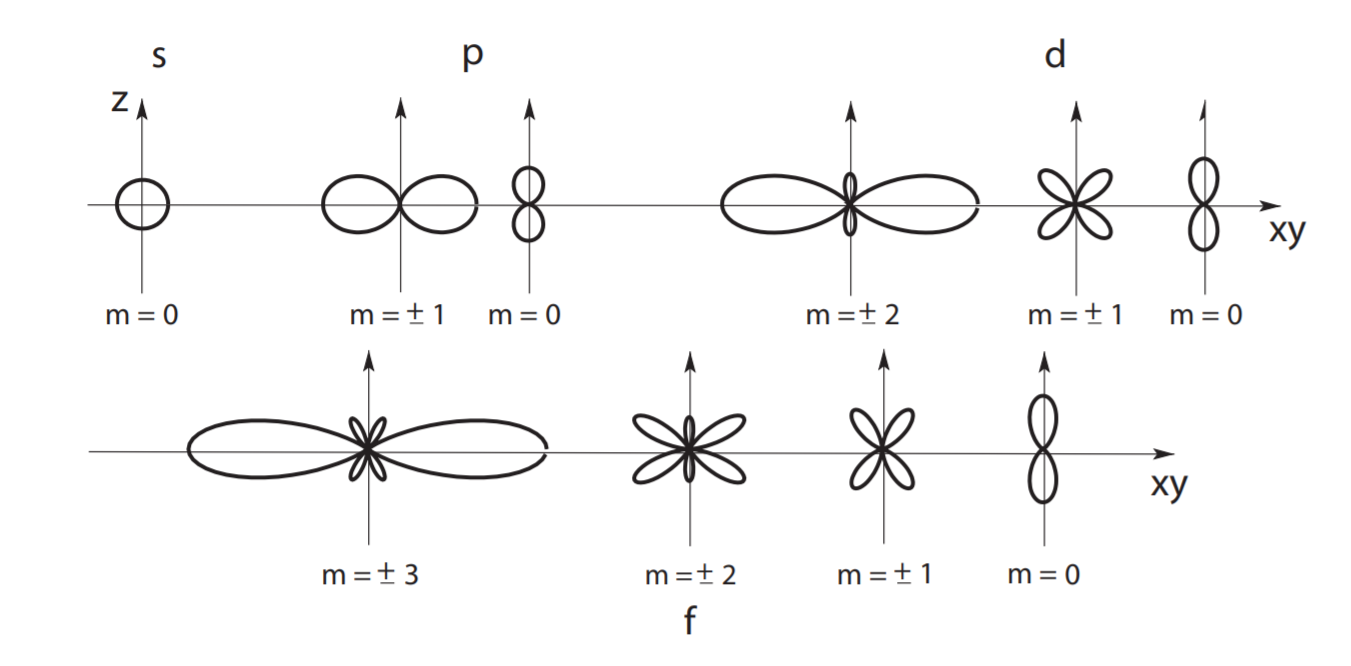
\includegraphics[scale=1]{4_5.PNG}
    \captionsetup{font={Large}}
    \caption{Polar diagrams $r = | Y_{lm} (\theta, \varphi = 0) |^2$ of the spherical functions to $l \leq 3$. The abbreviations $s, p, d, f$ refer to angular momenta with $l = 0, 1, 2, 3$.}
\end{figure}
It is $\langle l, m | L_x l,m\rangle \equiv \langle L_x\rangle_{lm} = \langle L_y\rangle_{lm} = 0$. The states $| l, \pm l\rangle$ are concentrated in the $xy$-plane with $\langle \Delta L_x\rangle_{u} = \langle L^2_x-\langle L_x\rangle^2_{u}\rangle^{1/2}_{u}=\langle L_x^2\rangle^{1/2}_{u}=\sqrt{l/2}\hbar$ and $\langle \Delta L_y\rangle_u=\sqrt{l/2}\hbar$. The states $| l, 0\rangle$ are along the $z$-axis
extended.\\\\
It is instructive to find the spherical functions $Y_{lm}$ as solutions of the eigenvalue problem to the operators $iL_z/\hbar=\partial_{\varphi}$ and $-L^2/\hbar^2=\Delta \operatorname{auf}\mathbb{L}_2(S^2)$. We first calculate the $\varphi$-dependence,
%公式 4:57
\begin{equation}
\begin{aligned} \partial_{\varphi} Y_{l m} &=i m Y_{l m} \\ \Rightarrow Y_{l m}(\theta, \varphi) &=e^{i m \varphi} p(\theta) \end{aligned}
\end{equation}
with $m$ completely such that $Y_{lm} (\theta, \varphi + 2\pi) = Y_{lm} (\theta, \varphi)$. Then we determine the $\theta$ dependence,
%公式 4:58
\begin{equation}
\begin{aligned} L^{2} Y_{l m}(\theta, \varphi) &=\hbar^{2} l(l+1) Y_{l m}(\theta, \varphi) \\\left[\frac{1}{\sin \theta} \partial_{\theta} \sin \theta \partial_{\theta}-\frac{m^{2}}{\sin ^{2} \theta}+l(l+1)\right] p(\theta) &=0 \end{aligned}
\end{equation}
or with $z = cos \theta$,
%公式 4:59
\begin{equation}
    \left[\partial_{z}\left[\left(1-z^{2}\right) \partial_{z}\right]-\frac{m^{2}}{1-z^{2}}+l(l+1)\right] p(z)=0
    \end{equation}
As a solution, we obtain the associated legendary functions, see (3.150). First, consider the case $m = 0$ and find the legend polynomials
%公式 4.60
\begin{equation}
\begin{aligned} p(z) &=P_{l}(z)=\left[2 l^{l} l ! !\right]^{-1} \partial_{z}^{l}\left(z^{2}-1\right)^{l} \\ P_{0}=1, \quad P_{1}=z, & P_{2}=\left(3 z^{2}-1\right) / 2, \quad P_{3}=\left(5 z^{3}-3 z\right) / 2, \cdots \end{aligned}
\end{equation}
with the properties
%公式 4.61
\begin{equation}
\begin{aligned}(l+1) P_{l+1} &=(2 l+1) z P_{l}-l P_{l-1} \\\left(1-z^{2}\right) \partial_{z} P_{l} &=l P_{l-1}-l z P_{l} \\ \int_{-1}^{1} d z P_{l}(z) P_{l^{\prime}}(z) &=\frac{2}{2 l+1} \delta_{l l^{\prime}} \end{aligned}
\end{equation}
Next we consider $m \neq 0$ arbitrarily and get the associated Legendre polynomials,
%公式 4.62
\begin{equation}
\begin{aligned} P_{l m}(z) &=\left(1-z^{2}\right)^{m / 2} \partial_{z}^{m} P_{l}(z), \quad m=0,1, \ldots, l \\ &=\left[2^{l} l !\right]^{-1}\left(1-z^{2}\right)^{m / 2} \partial_{z}^{l+m}\left(z^{2}-1\right)^{l}, \quad m=-l, \ldots, l \end{aligned}
\end{equation}
They have the properties (with $n !! = n (n - 2) (n - 4)\dots$)
%公式 4.63
\begin{equation}
\begin{aligned} P_{l m}(-z) &=(-1)^{l+m} P_{l m}(z) \\ P_{l 0}=P_{l}, & P_{l l}=(2 l-1) ! !\left(1-z^{2}\right)^{l / 2} \\(l+1-m) P_{l+1 m} &=(2 l+1) z P_{l m}-(l+m) P_{l-1 m} \\\left(1-z^{2}\right) \partial_{z} P_{l m} &=(l+m) P_{l-1 m}-l z P_{l m} \\ \int_{-1}^{1} d z P_{l m}(z) P_{l^{\prime} m}(z) &=\frac{2}{2 l+1} \frac{(l+m) !}{(l-m) !} \delta_{l l^{\prime}} \end{aligned}
\end{equation}
The combination of the above results gives us the spherical functions
%公式 4.64
\begin{equation}
    Y_{l m}(\theta, \varphi)=(-1)^{m} \sqrt{\frac{2 l+1}{4 \pi}} \frac{(l-m) !}{(l+m) !} e^{i m \varphi} P_{l m}(\cos \theta)
    \end{equation}

\section{Rotation and tensors}
In this section we set $\hbar= 1$. The rotation $U_{\vec{w}}=exp(-i\vec{w}\cdot\vec{L})$ rotates a state about the axis $\vec{w}$ with the angle $|\vec{w}|$; the rotation is positive (note $U_{\vec{a}}$ shifts a position by $\vec{a},U_{\vec{w}}$ turns a position by $\vec{w}$).\\\\
Let the eigenstate $l,m\rangle$ be rotated to $L^2$, $L_z$. $U_{\vec{w}}$ leaves $l$ invariant but generally mixes the $m$-values. As a result, is

%公式 4.65
\begin{equation}
    U_{\vec{\omega}}|l, m\rangle=\sum_{m^{\prime}=-l}^{l} d_{m^{\prime} m}^{l}(\vec{\omega})\left|l, m^{\prime}\right\rangle
    \end{equation}
The coefficient matrix $d^l_{m^{\prime}m}(\vec{w})$ is given by
%公式 4.66
\begin{equation}
\begin{aligned} d_{m^{\prime} m}^{l}(\vec{\omega}) &=\left\langle l, m^{\prime}\left|e^{-i \vec{\omega} \cdot \vec{L}}\right| l, m\right\rangle \\ &=\left[\mathcal{D}^{l}(\vec{\omega})\right]_{m^{\prime} m} \end{aligned}
\end{equation}
The matrices [$\mathcal{D}^l_{\vec{w}}$] define the $2l + 1$-dimensional irreducible representations of the rotation group $SO (3)$. The rotation matrices $\mathcal{D}$ are unitary, $\mathcal{D}^{\dagger}(\vec{w})\mathcal{D}(\vec{w})=\mathcal{D}(-\vec{w})\mathcal{D}(\vec{w}) = \mathbb{I}$, so $\mathcal{D}^{\dagger}(\vec{w})=\mathcal{D}(\vec{w})$, and in components, $[\mathcal{D}^{l\dagger}(\vec{w})]_{m^{\prime}m}=d^{l*}_{mm^{\prime}}(\vec{w})=d^l_{m^{\prime}m}(-\vec{w})$ To find the matrices $d^l_{m^{\prime}m}(\vec{w})$, we introduce the Euler angles, see fig. 4.6. Any
%图 4.6
\begin{figure}[ht]
    \begin{minipage}{0.55\textwidth}
        \centering
        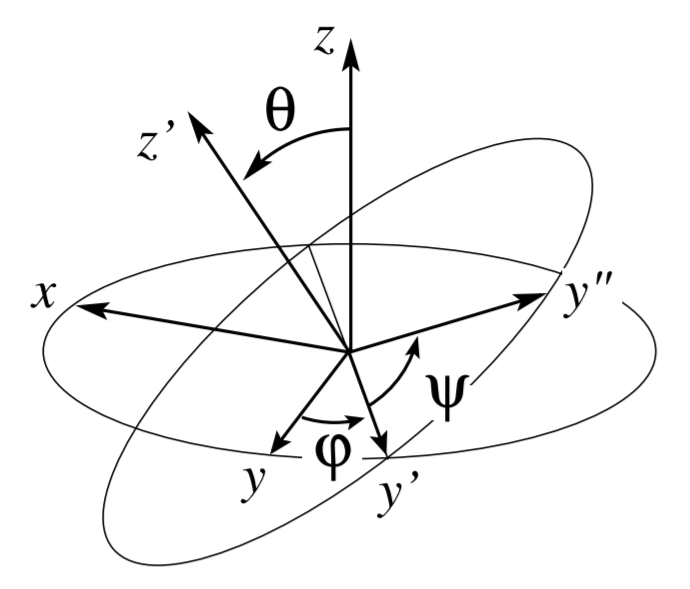
\includegraphics[scale=1]{4_6.PNG}
    \end{minipage}
    \begin{minipage}{0.45\textwidth}
        \captionsetup{font={Large}}
        \caption{Euler angle $\varphi$ (rotation around $z$, defined $y^{\prime}$), $\theta$ (rotation around $y^{\prime}$, defined $z^{\prime}$), $\phi$ (rotation around $z^{\prime}$, defined $y^{\prime\prime}$).}
    \end{minipage}
\end{figure}
Rotation $R (\varphi, \theta, \Psi)$ can be represented as a combination of single rotations with the help of Euler angles.
%公式 4.67
\begin{equation}
\begin{aligned} R(\varphi, \theta, \psi) & e^{-i \psi L_{z^{\prime}}} \quad e^{-i \theta L_{y^{\prime}}} \quad e^{-i \varphi L_{z}} \\ \text { Turn around } & z^{\prime}-\quad y^{\prime}-\quad z-\text { axis } \end{aligned}
\end{equation}
compare fig. 4.6. We use that
%公式 4.68
\begin{equation}
\begin{aligned} L_{y^{\prime}} &=e^{-i \varphi L_{z}} L_{y} e^{i \varphi L_{z}} \\ e^{-i \theta L_{y^{\prime}}} &=e^{-i \varphi L_{z}} e^{-i \theta L_{y}} e^{i \varphi L_{z}} \\ e^{-i \psi L_{z^{\prime}}} &=e^{-i \theta L_{y^{\prime}}} e^{-i \psi L_{z}} e^{i \theta L_{y^{\prime}}} \end{aligned}
\end{equation}
the use of these expressions in (4.67) yields
%公式 4.69
\begin{equation}
\begin{aligned} R(\varphi, \theta, \psi) &=e^{-i \theta L_{y^{\prime}}} e^{-i \psi L_{z}} e^{i \theta L_{y^{\prime}}} e^{-i \varphi L_{z}} e^{-i \theta L_{y}} \underbrace{e^{i \varphi L_{z}} e^{-i \varphi L_{z}}}_{1} \\ &=e^{-i \varphi L_{z}} e^{-i \theta L_{y}} e^{i \varphi L_{z}} e^{-i \psi L_{z}} e^{-i \varphi L_{z}} e^{i \theta L_{y}} e^{i \varphi L_{z}} e^{-i \varphi L_{z}} e^{-i \theta L_{y}} \\ &=e^{-i \varphi L_{z}} e^{-i \theta L_{y}} e^{-i \psi L_{z}} \end{aligned}
\end{equation}
Inserting (4.69) into the definition (4.66) yields for the coefficient matrix $d^l_{mm^{\prime}} (\varphi, \theta, \psi)$
%公式 4.70
\begin{equation}
\begin{aligned} d_{m m^{\prime}}^{l}(\varphi, \theta, \psi)=& e^{-i m \varphi} e^{-i m^{\prime} \psi} d_{m m^{\prime}}^{l}(\theta) \\ \text { mit } d_{m m^{\prime}}^{l}(\theta)=& \left\langle l, m\left|e^{-i \theta L_{y}}\right| l, m^{\prime}\right\rangle \end{aligned}
\end{equation}
The elements $d^l_{m^{\prime}}$ are easy to find: It is $|\theta,\varphi\rangle = R_{φ, \theta, 0} | \theta = 0, \varphi = 0\rangle$ and the projection on $\langle l, m |$ results
%公式 4.71
\begin{equation}
\begin{aligned}\langle l, m | \theta, \varphi\rangle=& \sum_{m^{\prime}}\left\langle l, m\left|R_{\varphi, \theta, 0}\right| l, m^{\prime}\right\rangle\left\langle l, m^{\prime} | 0,0\right\rangle \\ Y_{l m}^{*}(\theta, \varphi)=& \sum_{m^{\prime}} d_{m m^{\prime}}^{l}(\varphi, \theta, 0) \quad \underbrace{Y_{l, m^{\prime}}^{*}(0,0)}_{\delta_{m^{\prime}, 0} \sqrt{2 l+1 / 4 \pi}} \\ \Rightarrow & d_{m, 0}^{l}(\varphi, \theta, \psi)=\sqrt{\frac{4 \pi}{2 l+1}} Y_{l m}^{*}(\theta, \varphi) \end{aligned}
\end{equation}
The other elements $d^l_{mm^{\prime}}$ with $m^{\prime}\neq 0$ are a little harder to find; the result is (see exercises)
%公式 4.72
\begin{equation}
\begin{array}{l}{d_{m m^{\prime}}^{l}(\theta)=(-1)^{l+m^{\prime}}\left[\frac{\left(l+m^{\prime}\right) !}{\left(l-m^{\prime}\right) !(l+m) !(l-m) !}\right]^{1 / 2} \sin ^{m^{\prime}-m}(\theta / 2)} \\ {\times \cos ^{m+m^{\prime}}(\theta / 2)\left[(1-t)^{m-m^{\prime}} t^{-m-m^{\prime}} \partial_{t}^{l-m^{\prime}}\left[t^{l+m}(1-t)^{l-m}\right]\right]_{t=\cos ^{2} \frac{\theta}{2}}}\end{array}
\end{equation}
The $d^l_{mm^{\prime}}$ describe the transformation behavior of tensor operators under rotation: An irreducible tensor operator Tk of order $k$ with its $2k + 1$ components $T^k_q, q \in {-k, -k + 1, \dots, k-1, k}$ transforms under rotations according to
%公式 4.73
\begin{equation}
    U_{\vec{\omega}} T_{q}^{k} U_{\vec{\omega}}^{-1}=\sum_{q^{\prime}=-k}^{k} d_{q^{\prime} q}^{k}(\vec{\omega}) T_{q^{\prime}}^{k}
    \end{equation}
The relation (4.73) is the defining property of a 'rotation tensor' $T^k$. Knowing the behavior (4.73) under rotations allows us to easily calculate the commutators $[\vec{L}, T^k_q]$: For small $\vec{w}$ is $U_{\vec{w}}\approx \mathbb{I}-i\vec{w}\cdot\vec{L}$ and we get
%公式 4.74
\begin{equation}
\begin{aligned}
    \left[\vec{L}, T_{q}^{k}\right] &=\sum_{q^{\prime}}\left\langle k, q^{\prime}|\vec{L}| k, q\right\rangle T_{q^{\prime}}^{k} 
\end{aligned}
\end{equation}
%公式 4.75
\begin{equation}
    \left[L_{z}, T_{q}^{k}\right] =q T_{q}^{k} 
\end{equation}
%公式 4.76
\begin{equation}
    \left[L_{\pm}, T_{q}^{k}\right] =\sqrt{k(k+1)-q(q \pm 1)} T_{q \pm 1}^{k} 
\end{equation}
For $k = 0$ we obtain a scalar operator $S$ with the transformation behavior (use that $d^0_{00} = 1$)
%公式 4.77
\begin{equation}
    S \rightarrow S^{\prime}=U_{\vec{\omega}} S U_{\vec{\omega}}^{-1}=S
    \end{equation}
that is, a scalar is invariant under rotation.
The superscript $k = 1$ denotes a vector operator $\vec{V}$ with 3 components, e.g. $\vec{r},\vec{p},\vec{L}$. The $q$-components of $V ~$ are

%公式 4.78
\begin{equation}
    V_{q=0}=V_{z}, V_{q=\pm 1}=\mp \frac{1}{\sqrt{2}}\left(V_{x} \pm i V_{y}\right)
    \end{equation}
For vector operators $\vec{V}$ in Cartesian components, we have previously found that
%公式 4.79
\begin{equation}
    \left[L_{i}, V_{j}\right]=i \varepsilon_{i j k} V_{k}, \quad i, j, k \doteq x, y, z
    \end{equation}
The results (4.74) and (4.79) are equivalent with the help of (4.78).
An example of a second-order tensor operator can be constructed as follows: Let $\vec{U}$ and $\vec{V}$ be two vectors. We group the components of the direct product accordingly
%公式
\begin{equation}
    V_{i} U_{j}=\underbrace{\frac{\vec{V} \cdot \vec{U}}{3} \delta_{i j}}_{\rightarrow \text { scalar }}+\underbrace{\frac{V_{i} U_{j}-U_{i} V_{j}}{2}}_{\frac{1}{2} \varepsilon_{i j k}(\vec{V} \wedge \vec{U})_{k} \rightarrow \text { vector }}+\underbrace{\left(\frac{V_{i} U_{j}+U_{i} V_{j}}{2}-\frac{\vec{V} \cdot \vec{U}}{3} \delta_{i j}\right)}_{\rightarrow \text { tensor 2nd order }}
    \end{equation}
We print the 5 components $T_{ij}$ of this tensor $(T_{ij} = T_{ji}, \operatorname{Sp}T = 0)$ in rotational components $T^k_{\pm q}$,
%公式
%公式 4.80
\begin{equation}
    \begin{aligned} 
    T_{0}^{2} =& \frac{1}{\sqrt{6}}\left(V_{1} U_{-1}+2 V_{0} U_{0}+V_{-1} U_{1}\right) \\ 
    T_{\pm 1}^{2} =& \frac{1}{\sqrt{2}}\left(V_{\pm 1} U_{0}+V_{0} U_{\pm 1}\right) \\ 
    T_{\pm 2}^{2} =& V_{\pm 1} U_{\pm 1}
    \end{aligned}
\end{equation}\\
For more details, see Gordon Baym, chapter 17.

\newpage